\documentclass[12pt]{article}
\usepackage{enumerate}
\usepackage{mathematics}

\DeclareMathOperator{\diam}{\mathrm{diam}}


\begin{document}

\title{Oxford M5 - Multivariable Calculus
  \footnotetext{\url{https://courses.maths.ox.ac.uk/node/5652}}}
\author{}
\date{}
\maketitle


\section{}

\begin{mdframed}
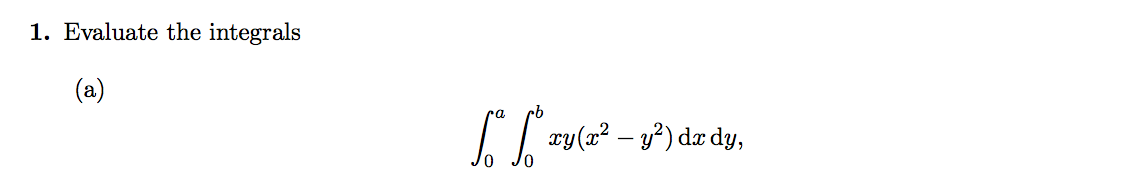
\includegraphics[width=400pt]{img/oxford-prelims-M5-multivariable-calc-1-1-a.png}
\end{mdframed}

\begin{align*}
  \int_0^a\int_0^b xy(x^2 - y^2)\dx\dy
  &= \int_0^a\int_0^b x^3y - xy^3\dx\dy\\
  &= \int_0^a\frac{b^4}{4}y - \frac{b^2}{2}y^3\dy\\
  &= \frac{a^2b^4}{8} - \frac{a^4b^2}{8} \checkmark
\end{align*}

\begin{mdframed}
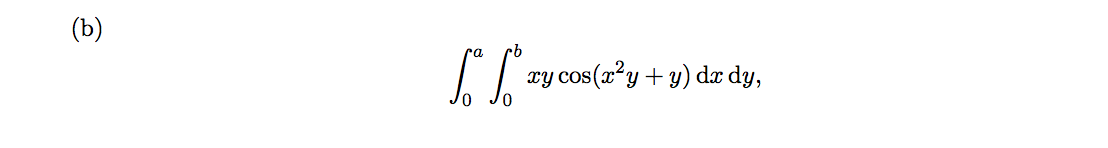
\includegraphics[width=400pt]{img/oxford-prelims-M5-multivariable-calc-1-1-b.png}
\end{mdframed}

\begin{align*}
  \int_0^a\int_0^b xy\cos(x^2y + y)\dx\dy
  &= \int_0^a \frac{1}{2}\sin(b^2y + y) \dy\\
  &= \frac{-\cos(a(b^2 + 1))}{2(b^2 + 1)}
\end{align*}

\begin{mdframed}
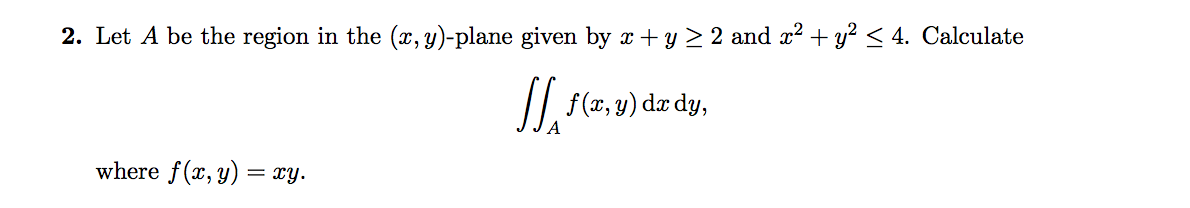
\includegraphics[width=400pt]{img/oxford-prelims-M5-multivariable-calc-1-2.png}
\end{mdframed}

\begin{mdframed}
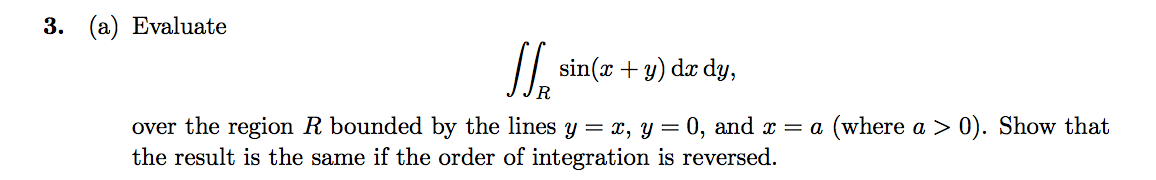
\includegraphics[width=400pt]{img/oxford-prelims-M5-multivariable-calc-1-3-a.png}
\end{mdframed}

\begin{mdframed}
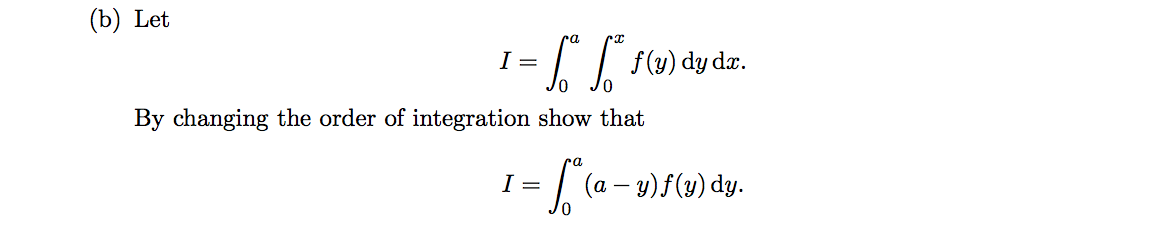
\includegraphics[width=400pt]{img/oxford-prelims-M5-multivariable-calc-1-3-b.png}
\end{mdframed}

\begin{mdframed}
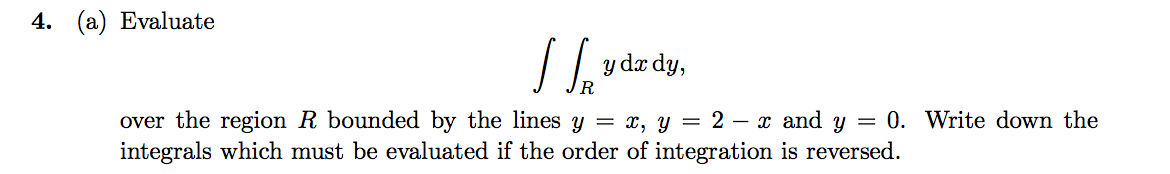
\includegraphics[width=400pt]{img/oxford-prelims-M5-multivariable-calc-1-4-a.png}
\end{mdframed}

\begin{mdframed}
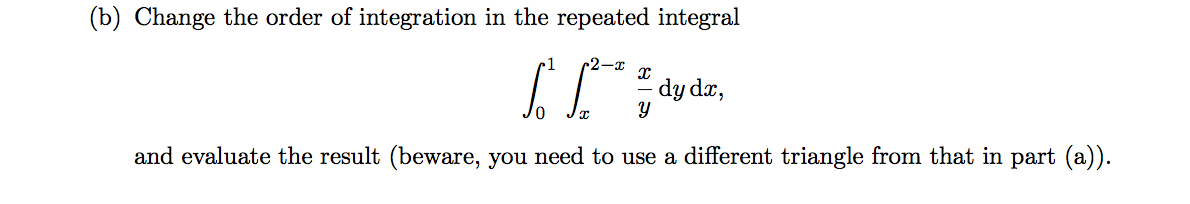
\includegraphics[width=400pt]{img/oxford-prelims-M5-multivariable-calc-1-4-b.png}
\end{mdframed}

\end{document}
